\documentclass[1p]{elsarticle_modified}
%\bibliographystyle{elsarticle-num}

%\usepackage[colorlinks]{hyperref}
%\usepackage{abbrmath_seonhwa} %\Abb, \Ascr, \Acal ,\Abf, \Afrak
\usepackage{amsfonts}
\usepackage{amssymb}
\usepackage{amsmath}
\usepackage{amsthm}
\usepackage{scalefnt}
\usepackage{amsbsy}
\usepackage{kotex}
\usepackage{caption}
\usepackage{subfig}
\usepackage{color}
\usepackage{graphicx}
\usepackage{xcolor} %% white, black, red, green, blue, cyan, magenta, yellow
\usepackage{float}
\usepackage{setspace}
\usepackage{hyperref}

\usepackage{tikz}
\usetikzlibrary{arrows}

\usepackage{multirow}
\usepackage{array} % fixed length table
\usepackage{hhline}

%%%%%%%%%%%%%%%%%%%%%
\makeatletter
\renewcommand*\env@matrix[1][\arraystretch]{%
	\edef\arraystretch{#1}%
	\hskip -\arraycolsep
	\let\@ifnextchar\new@ifnextchar
	\array{*\c@MaxMatrixCols c}}
\makeatother %https://tex.stackexchange.com/questions/14071/how-can-i-increase-the-line-spacing-in-a-matrix
%%%%%%%%%%%%%%%

\usepackage[normalem]{ulem}

\newcommand{\msout}[1]{\ifmmode\text{\sout{\ensuremath{#1}}}\else\sout{#1}\fi}
%SOURCE: \msout is \stkout macro in https://tex.stackexchange.com/questions/20609/strikeout-in-math-mode

\newcommand{\cancel}[1]{
	\ifmmode
	{\color{red}\msout{#1}}
	\else
	{\color{red}\sout{#1}}
	\fi
}

\newcommand{\add}[1]{
	{\color{blue}\uwave{#1}}
}

\newcommand{\replace}[2]{
	\ifmmode
	{\color{red}\msout{#1}}{\color{blue}\uwave{#2}}
	\else
	{\color{red}\sout{#1}}{\color{blue}\uwave{#2}}
	\fi
}

\newcommand{\Sol}{\mathcal{S}} %segment
\newcommand{\D}{D} %diagram
\newcommand{\A}{\mathcal{A}} %arc


%%%%%%%%%%%%%%%%%%%%%%%%%%%%%5 test

\def\sl{\operatorname{\textup{SL}}(2,\Cbb)}
\def\psl{\operatorname{\textup{PSL}}(2,\Cbb)}
\def\quan{\mkern 1mu \triangleright \mkern 1mu}

\theoremstyle{definition}
\newtheorem{thm}{Theorem}[section]
\newtheorem{prop}[thm]{Proposition}
\newtheorem{lem}[thm]{Lemma}
\newtheorem{ques}[thm]{Question}
\newtheorem{cor}[thm]{Corollary}
\newtheorem{defn}[thm]{Definition}
\newtheorem{exam}[thm]{Example}
\newtheorem{rmk}[thm]{Remark}
\newtheorem{alg}[thm]{Algorithm}

\newcommand{\I}{\sqrt{-1}}
\begin{document}

%\begin{frontmatter}
%
%\title{Boundary parabolic representations of knots up to 8 crossings}
%
%%% Group authors per affiliation:
%\author{Yunhi Cho} 
%\address{Department of Mathematics, University of Seoul, Seoul, Korea}
%\ead{yhcho@uos.ac.kr}
%
%
%\author{Seonhwa Kim} %\fnref{s_kim}}
%\address{Center for Geometry and Physics, Institute for Basic Science, Pohang, 37673, Korea}
%\ead{ryeona17@ibs.re.kr}
%
%\author{Hyuk Kim}
%\address{Department of Mathematical Sciences, Seoul National University, Seoul 08826, Korea}
%\ead{hyukkim@snu.ac.kr}
%
%\author{Seokbeom Yoon}
%\address{Department of Mathematical Sciences, Seoul National University, Seoul, 08826,  Korea}
%\ead{sbyoon15@snu.ac.kr}
%
%\begin{abstract}
%We find all boundary parabolic representation of knots up to 8 crossings.
%
%\end{abstract}
%\begin{keyword}
%    \MSC[2010] 57M25 
%\end{keyword}
%
%\end{frontmatter}

%\linenumbers
%\tableofcontents
%
\newcommand\colored[1]{\textcolor{white}{\rule[-0.35ex]{0.8em}{1.4ex}}\kern-0.8em\color{red} #1}%
%\newcommand\colored[1]{\textcolor{white}{ #1}\kern-2.17ex	\textcolor{white}{ #1}\kern-1.81ex	\textcolor{white}{ #1}\kern-2.15ex\color{red}#1	}

{\Large $\underline{12a_{0372}~(K12a_{0372})}$}

\setlength{\tabcolsep}{10pt}
\renewcommand{\arraystretch}{1.6}
\vspace{1cm}\begin{tabular}{m{100pt}>{\centering\arraybackslash}m{274pt}}
\multirow{5}{120pt}{
	\centering
	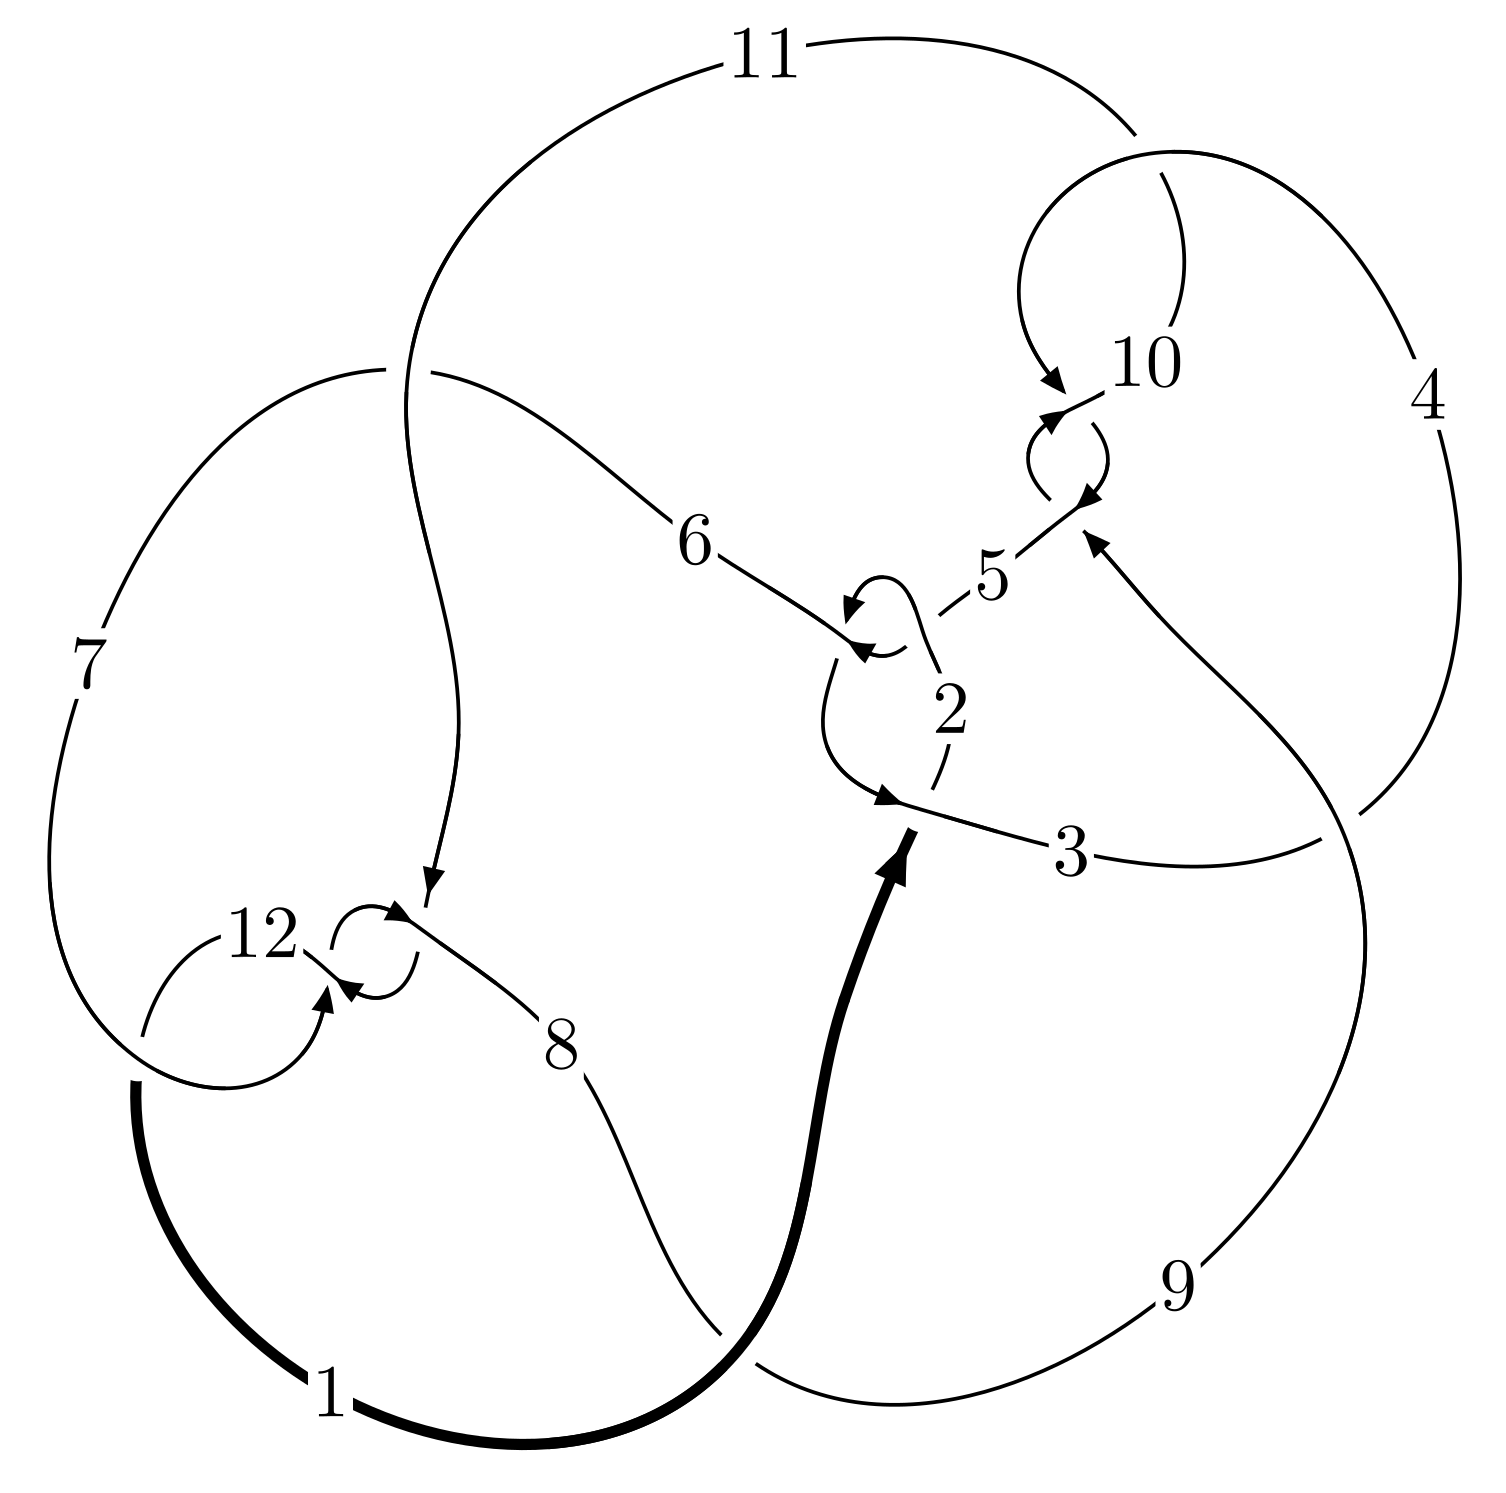
\includegraphics[width=112pt]{../../../GIT/diagram.site/Diagrams/png/1173_12a_0372.png}\\
\ \ \ A knot diagram\footnotemark}&
\allowdisplaybreaks
\textbf{Linearized knot diagam} \\
\cline{2-2}
 &
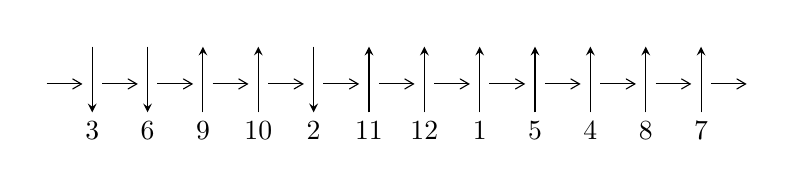
\begin{tikzpicture}[x=20pt, y=17pt]
	% nodes
	\node (C0) at (0, 0) {};
	\node (C1) at (1, 0) {};
	\node (C1U) at (1, +1) {};
	\node (C1D) at (1, -1) {3};

	\node (C2) at (2, 0) {};
	\node (C2U) at (2, +1) {};
	\node (C2D) at (2, -1) {6};

	\node (C3) at (3, 0) {};
	\node (C3U) at (3, +1) {};
	\node (C3D) at (3, -1) {9};

	\node (C4) at (4, 0) {};
	\node (C4U) at (4, +1) {};
	\node (C4D) at (4, -1) {10};

	\node (C5) at (5, 0) {};
	\node (C5U) at (5, +1) {};
	\node (C5D) at (5, -1) {2};

	\node (C6) at (6, 0) {};
	\node (C6U) at (6, +1) {};
	\node (C6D) at (6, -1) {11};

	\node (C7) at (7, 0) {};
	\node (C7U) at (7, +1) {};
	\node (C7D) at (7, -1) {12};

	\node (C8) at (8, 0) {};
	\node (C8U) at (8, +1) {};
	\node (C8D) at (8, -1) {1};

	\node (C9) at (9, 0) {};
	\node (C9U) at (9, +1) {};
	\node (C9D) at (9, -1) {5};

	\node (C10) at (10, 0) {};
	\node (C10U) at (10, +1) {};
	\node (C10D) at (10, -1) {4};

	\node (C11) at (11, 0) {};
	\node (C11U) at (11, +1) {};
	\node (C11D) at (11, -1) {8};

	\node (C12) at (12, 0) {};
	\node (C12U) at (12, +1) {};
	\node (C12D) at (12, -1) {7};
	\node (C13) at (13, 0) {};

	% arrows
	\draw[->,>={angle 60}]
	(C0) edge (C1) (C1) edge (C2) (C2) edge (C3) (C3) edge (C4) (C4) edge (C5) (C5) edge (C6) (C6) edge (C7) (C7) edge (C8) (C8) edge (C9) (C9) edge (C10) (C10) edge (C11) (C11) edge (C12) (C12) edge (C13) ;	\draw[->,>=stealth]
	(C1U) edge (C1D) (C2U) edge (C2D) (C3D) edge (C3U) (C4D) edge (C4U) (C5U) edge (C5D) (C6D) edge (C6U) (C7D) edge (C7U) (C8D) edge (C8U) (C9D) edge (C9U) (C10D) edge (C10U) (C11D) edge (C11U) (C12D) edge (C12U) ;
	\end{tikzpicture} \\
\hhline{~~} \\& 
\textbf{Solving Sequence} \\ \cline{2-2} 
 &
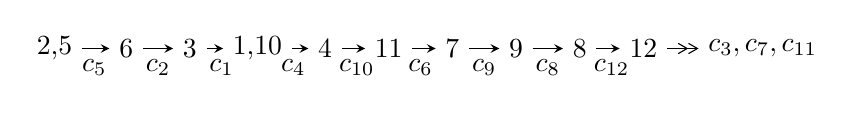
\begin{tikzpicture}[x=23pt, y=7pt]
	% node
	\node (A0) at (-1/8, 0) {2,5};
	\node (A1) at (1, 0) {6};
	\node (A2) at (2, 0) {3};
	\node (A3) at (49/16, 0) {1,10};
	\node (A4) at (33/8, 0) {4};
	\node (A5) at (41/8, 0) {11};
	\node (A6) at (49/8, 0) {7};
	\node (A7) at (57/8, 0) {9};
	\node (A8) at (65/8, 0) {8};
	\node (A9) at (73/8, 0) {12};
	\node (C1) at (1/2, -1) {$c_{5}$};
	\node (C2) at (3/2, -1) {$c_{2}$};
	\node (C3) at (5/2, -1) {$c_{1}$};
	\node (C4) at (29/8, -1) {$c_{4}$};
	\node (C5) at (37/8, -1) {$c_{10}$};
	\node (C6) at (45/8, -1) {$c_{6}$};
	\node (C7) at (53/8, -1) {$c_{9}$};
	\node (C8) at (61/8, -1) {$c_{8}$};
	\node (C9) at (69/8, -1) {$c_{12}$};
	\node (A10) at (11, 0) {$c_{3},c_{7},c_{11}$};

	% edge
	\draw[->,>=stealth]	
	(A0) edge (A1) (A1) edge (A2) (A2) edge (A3) (A3) edge (A4) (A4) edge (A5) (A5) edge (A6) (A6) edge (A7) (A7) edge (A8) (A8) edge (A9) ;
	\draw[->>,>={angle 60}]	
	(A9) edge (A10);
\end{tikzpicture} \\ 

\end{tabular} \\

\footnotetext{
The image of knot diagram is generated by the software ``\textbf{Draw programme}" developed by Andrew Bartholomew(\url{http://www.layer8.co.uk/maths/draw/index.htm\#Running-draw}), where we modified some parts for our purpose(\url{https://github.com/CATsTAILs/LinksPainter}).
}\phantom \\ \newline 
\centering \textbf{Ideals for irreducible components\footnotemark of $X_{\text{par}}$} 
 
\begin{align*}
I^u_{1}&=\langle 
-4.00775\times10^{87} u^{85}-2.48507\times10^{88} u^{84}+\cdots+1.44535\times10^{88} b+2.76929\times10^{89},\\
\phantom{I^u_{1}}&\phantom{= \langle  }-3.45221\times10^{89} u^{85}-1.15168\times10^{90} u^{84}+\cdots+4.91419\times10^{89} a+4.17969\times10^{90},\\
\phantom{I^u_{1}}&\phantom{= \langle  }u^{86}+4 u^{85}+\cdots-20 u-17\rangle \\
I^u_{2}&=\langle 
-194 a^5-315 a^4-5270 a^3-4555 a^2+69650 b-64279 a-26651,\\
\phantom{I^u_{2}}&\phantom{= \langle  }a^6+2 a^5+25 a^4+30 a^3+206 a^2+176 a+593,\;u-1\rangle \\
I^u_{3}&=\langle 
b,\;a^3+a^2-1,\;u+1\rangle \\
\\
\end{align*}
\raggedright * 3 irreducible components of $\dim_{\mathbb{C}}=0$, with total 95 representations.\\
\footnotetext{All coefficients of polynomials are rational numbers. But the coefficients are sometimes approximated in decimal forms when there is not enough margin.}
\newpage
\renewcommand{\arraystretch}{1}
\centering \section*{I. $I^u_{1}= \langle -4.01\times10^{87} u^{85}-2.49\times10^{88} u^{84}+\cdots+1.45\times10^{88} b+2.77\times10^{89},\;-3.45\times10^{89} u^{85}-1.15\times10^{90} u^{84}+\cdots+4.91\times10^{89} a+4.18\times10^{90},\;u^{86}+4 u^{85}+\cdots-20 u-17 \rangle$}
\flushleft \textbf{(i) Arc colorings}\\
\begin{tabular}{m{7pt} m{180pt} m{7pt} m{180pt} }
\flushright $a_{2}=$&$\begin{pmatrix}0\\u\end{pmatrix}$ \\
\flushright $a_{5}=$&$\begin{pmatrix}1\\0\end{pmatrix}$ \\
\flushright $a_{6}=$&$\begin{pmatrix}1\\u^2\end{pmatrix}$ \\
\flushright $a_{3}=$&$\begin{pmatrix}- u\\- u^3+u\end{pmatrix}$ \\
\flushright $a_{1}=$&$\begin{pmatrix}u^3\\u^5- u^3+u\end{pmatrix}$ \\
\flushright $a_{10}=$&$\begin{pmatrix}0.702499 u^{85}+2.34358 u^{84}+\cdots-17.6252 u-8.50536\\0.277286 u^{85}+1.71936 u^{84}+\cdots+8.31636 u-19.1600\end{pmatrix}$ \\
\flushright $a_{4}=$&$\begin{pmatrix}0.504301 u^{85}+1.30510 u^{84}+\cdots-13.8214 u-5.82459\\0.0137884 u^{85}+0.0233804 u^{84}+\cdots+1.94469 u-3.22686\end{pmatrix}$ \\
\flushright $a_{11}=$&$\begin{pmatrix}0.294534 u^{85}+1.15575 u^{84}+\cdots+5.28585 u-19.1152\\0.244106 u^{85}+0.263311 u^{84}+\cdots-4.48711 u+4.51370\end{pmatrix}$ \\
\flushright $a_{7}=$&$\begin{pmatrix}-1.36374 u^{85}-4.50519 u^{84}+\cdots+9.32384 u+28.0444\\0.448009 u^{85}+1.37637 u^{84}+\cdots-4.79587 u-5.94786\end{pmatrix}$ \\
\flushright $a_{9}=$&$\begin{pmatrix}0.425213 u^{85}+0.624223 u^{84}+\cdots-25.9416 u+10.6546\\0.277286 u^{85}+1.71936 u^{84}+\cdots+8.31636 u-19.1600\end{pmatrix}$ \\
\flushright $a_{8}=$&$\begin{pmatrix}-0.00970161 u^{85}-0.280717 u^{84}+\cdots-21.0594 u+11.2096\\0.0519514 u^{85}+0.807957 u^{84}+\cdots+2.49003 u-10.0728\end{pmatrix}$ \\
\flushright $a_{12}=$&$\begin{pmatrix}-1.53639 u^{85}-4.66319 u^{84}+\cdots+30.2188 u+12.1772\\0.253558 u^{85}+0.199433 u^{84}+\cdots-14.9224 u+12.1204\end{pmatrix}$\\&\end{tabular}
\flushleft \textbf{(ii) Obstruction class $= -1$}\\~\\
\flushleft \textbf{(iii) Cusp Shapes $= -0.907710 u^{85}-2.76373 u^{84}+\cdots+58.7556 u+7.47521$}\\~\\
\newpage\renewcommand{\arraystretch}{1}
\flushleft \textbf{(iv) u-Polynomials at the component}\newline \\
\begin{tabular}{m{50pt}|m{274pt}}
Crossings & \hspace{64pt}u-Polynomials at each crossing \\
\hline $$\begin{aligned}c_{1}\end{aligned}$$&$\begin{aligned}
&u^{86}+42 u^{85}+\cdots+8016 u+289
\end{aligned}$\\
\hline $$\begin{aligned}c_{2},c_{5}\end{aligned}$$&$\begin{aligned}
&u^{86}+4 u^{85}+\cdots-20 u-17
\end{aligned}$\\
\hline $$\begin{aligned}c_{3}\end{aligned}$$&$\begin{aligned}
&u^{86}- u^{85}+\cdots-8992 u+16424
\end{aligned}$\\
\hline $$\begin{aligned}c_{4},c_{9},c_{10}\end{aligned}$$&$\begin{aligned}
&u^{86}+u^{85}+\cdots+16 u+8
\end{aligned}$\\
\hline $$\begin{aligned}c_{6},c_{8}\end{aligned}$$&$\begin{aligned}
&u^{86}+2 u^{85}+\cdots-11367 u-2391
\end{aligned}$\\
\hline $$\begin{aligned}c_{7},c_{11},c_{12}\end{aligned}$$&$\begin{aligned}
&u^{86}-2 u^{85}+\cdots-3 u-3
\end{aligned}$\\
\hline
\end{tabular}\\~\\
\newpage\renewcommand{\arraystretch}{1}
\flushleft \textbf{(v) Riley Polynomials at the component}\newline \\
\begin{tabular}{m{50pt}|m{274pt}}
Crossings & \hspace{64pt}Riley Polynomials at each crossing \\
\hline $$\begin{aligned}c_{1}\end{aligned}$$&$\begin{aligned}
&y^{86}+14 y^{85}+\cdots-19463568 y+83521
\end{aligned}$\\
\hline $$\begin{aligned}c_{2},c_{5}\end{aligned}$$&$\begin{aligned}
&y^{86}-42 y^{85}+\cdots-8016 y+289
\end{aligned}$\\
\hline $$\begin{aligned}c_{3}\end{aligned}$$&$\begin{aligned}
&y^{86}-5 y^{85}+\cdots-1234215040 y+269747776
\end{aligned}$\\
\hline $$\begin{aligned}c_{4},c_{9},c_{10}\end{aligned}$$&$\begin{aligned}
&y^{86}+79 y^{85}+\cdots-1280 y+64
\end{aligned}$\\
\hline $$\begin{aligned}c_{6},c_{8}\end{aligned}$$&$\begin{aligned}
&y^{86}-56 y^{85}+\cdots+68087067 y+5716881
\end{aligned}$\\
\hline $$\begin{aligned}c_{7},c_{11},c_{12}\end{aligned}$$&$\begin{aligned}
&y^{86}+72 y^{85}+\cdots+51 y+9
\end{aligned}$\\
\hline
\end{tabular}\\~\\
\newpage\flushleft \textbf{(vi) Complex Volumes and Cusp Shapes}
$$\begin{array}{c|c|c}  
\text{Solutions to }I^u_{1}& \I (\text{vol} + \sqrt{-1}CS) & \text{Cusp shape}\\
 \hline 
\begin{aligned}
u &= \phantom{-}0.509248 + 0.852642 I \\
a &= \phantom{-}0.322825 + 0.048607 I \\
b &= -0.789445 - 0.160402 I\end{aligned}
 & \phantom{-}6.59236 + 1.97479 I & \phantom{-0.000000 } 0 \\ \hline\begin{aligned}
u &= \phantom{-}0.509248 - 0.852642 I \\
a &= \phantom{-}0.322825 - 0.048607 I \\
b &= -0.789445 + 0.160402 I\end{aligned}
 & \phantom{-}6.59236 - 1.97479 I & \phantom{-0.000000 } 0 \\ \hline\begin{aligned}
u &= \phantom{-}0.584122 + 0.824498 I \\
a &= -0.334198 - 0.153374 I \\
b &= \phantom{-}0.790561 + 0.106022 I\end{aligned}
 & \phantom{-}3.13486 - 2.30297 I & \phantom{-0.000000 } 0 \\ \hline\begin{aligned}
u &= \phantom{-}0.584122 - 0.824498 I \\
a &= -0.334198 + 0.153374 I \\
b &= \phantom{-}0.790561 - 0.106022 I\end{aligned}
 & \phantom{-}3.13486 + 2.30297 I & \phantom{-0.000000 } 0 \\ \hline\begin{aligned}
u &= -0.329631 + 0.932362 I \\
a &= -0.451079 - 0.979419 I \\
b &= \phantom{-}0.32373 - 1.38168 I\end{aligned}
 & -2.75721 - 10.22800 I & \phantom{-0.000000 } 0 \\ \hline\begin{aligned}
u &= -0.329631 - 0.932362 I \\
a &= -0.451079 + 0.979419 I \\
b &= \phantom{-}0.32373 + 1.38168 I\end{aligned}
 & -2.75721 + 10.22800 I & \phantom{-0.000000 } 0 \\ \hline\begin{aligned}
u &= \phantom{-}0.896991 + 0.410818 I \\
a &= \phantom{-}0.53853 + 2.78692 I \\
b &= \phantom{-}0.06533 + 1.51526 I\end{aligned}
 & -4.54753 - 1.67750 I & \phantom{-0.000000 } 0 \\ \hline\begin{aligned}
u &= \phantom{-}0.896991 - 0.410818 I \\
a &= \phantom{-}0.53853 - 2.78692 I \\
b &= \phantom{-}0.06533 - 1.51526 I\end{aligned}
 & -4.54753 + 1.67750 I & \phantom{-0.000000 } 0 \\ \hline\begin{aligned}
u &= -0.371807 + 0.912630 I \\
a &= \phantom{-}0.399618 + 0.904183 I \\
b &= -0.326539 + 1.355580 I\end{aligned}
 & \phantom{-}1.81661 - 5.99490 I & \phantom{-0.000000 } 0 \\ \hline\begin{aligned}
u &= -0.371807 - 0.912630 I \\
a &= \phantom{-}0.399618 - 0.904183 I \\
b &= -0.326539 - 1.355580 I\end{aligned}
 & \phantom{-}1.81661 + 5.99490 I & \phantom{-0.000000 } 0\\
 \hline 
 \end{array}$$\newpage$$\begin{array}{c|c|c}  
\text{Solutions to }I^u_{1}& \I (\text{vol} + \sqrt{-1}CS) & \text{Cusp shape}\\
 \hline 
\begin{aligned}
u &= \phantom{-}0.447851 + 0.874871 I \\
a &= -0.312467 + 0.033097 I \\
b &= \phantom{-}0.787438 + 0.204817 I\end{aligned}
 & \phantom{-}2.26451 + 6.21660 I & \phantom{-0.000000 } 0 \\ \hline\begin{aligned}
u &= \phantom{-}0.447851 - 0.874871 I \\
a &= -0.312467 - 0.033097 I \\
b &= \phantom{-}0.787438 - 0.204817 I\end{aligned}
 & \phantom{-}2.26451 - 6.21660 I & \phantom{-0.000000 } 0 \\ \hline\begin{aligned}
u &= -0.608566 + 0.769255 I \\
a &= -0.650245 + 0.848054 I \\
b &= \phantom{-}0.384469 + 0.945216 I\end{aligned}
 & -0.04968 - 1.95533 I & \phantom{-0.000000 } 0 \\ \hline\begin{aligned}
u &= -0.608566 - 0.769255 I \\
a &= -0.650245 - 0.848054 I \\
b &= \phantom{-}0.384469 - 0.945216 I\end{aligned}
 & -0.04968 + 1.95533 I & \phantom{-0.000000 } 0 \\ \hline\begin{aligned}
u &= -0.428356 + 0.876203 I \\
a &= -0.326362 - 0.791803 I \\
b &= \phantom{-}0.324167 - 1.315440 I\end{aligned}
 & -1.30715 - 1.70626 I & \phantom{-0.000000 } 0 \\ \hline\begin{aligned}
u &= -0.428356 - 0.876203 I \\
a &= -0.326362 + 0.791803 I \\
b &= \phantom{-}0.324167 + 1.315440 I\end{aligned}
 & -1.30715 + 1.70626 I & \phantom{-0.000000 } 0 \\ \hline\begin{aligned}
u &= -0.686031 + 0.768487 I \\
a &= \phantom{-}0.752897 - 0.902852 I \\
b &= -0.373726 - 1.024720 I\end{aligned}
 & \phantom{-}3.93150 + 2.25304 I & \phantom{-0.000000 } 0 \\ \hline\begin{aligned}
u &= -0.686031 - 0.768487 I \\
a &= \phantom{-}0.752897 + 0.902852 I \\
b &= -0.373726 + 1.024720 I\end{aligned}
 & \phantom{-}3.93150 - 2.25304 I & \phantom{-0.000000 } 0 \\ \hline\begin{aligned}
u &= \phantom{-}0.924737 + 0.534530 I \\
a &= \phantom{-}0.575892 + 0.848478 I \\
b &= -0.665118 + 0.182466 I\end{aligned}
 & \phantom{-}0.27137 - 3.73444 I & \phantom{-0.000000 } 0 \\ \hline\begin{aligned}
u &= \phantom{-}0.924737 - 0.534530 I \\
a &= \phantom{-}0.575892 - 0.848478 I \\
b &= -0.665118 - 0.182466 I\end{aligned}
 & \phantom{-}0.27137 + 3.73444 I & \phantom{-0.000000 } 0\\
 \hline 
 \end{array}$$\newpage$$\begin{array}{c|c|c}  
\text{Solutions to }I^u_{1}& \I (\text{vol} + \sqrt{-1}CS) & \text{Cusp shape}\\
 \hline 
\begin{aligned}
u &= \phantom{-}0.966175 + 0.460720 I \\
a &= -0.52607 - 2.70537 I \\
b &= -0.09038 - 1.52749 I\end{aligned}
 & -8.90441 - 5.42664 I & \phantom{-0.000000 } 0 \\ \hline\begin{aligned}
u &= \phantom{-}0.966175 - 0.460720 I \\
a &= -0.52607 + 2.70537 I \\
b &= -0.09038 + 1.52749 I\end{aligned}
 & -8.90441 + 5.42664 I & \phantom{-0.000000 } 0 \\ \hline\begin{aligned}
u &= -0.756050 + 0.766739 I \\
a &= -0.861234 + 0.982031 I \\
b &= \phantom{-}0.371400 + 1.094440 I\end{aligned}
 & \phantom{-}0.10136 + 6.51112 I & \phantom{-0.000000 } 0 \\ \hline\begin{aligned}
u &= -0.756050 - 0.766739 I \\
a &= -0.861234 - 0.982031 I \\
b &= \phantom{-}0.371400 - 1.094440 I\end{aligned}
 & \phantom{-}0.10136 - 6.51112 I & \phantom{-0.000000 } 0 \\ \hline\begin{aligned}
u &= -0.986156 + 0.463423 I \\
a &= \phantom{-}2.45774 - 1.20507 I \\
b &= -0.189677 - 1.345070 I\end{aligned}
 & -8.83115 + 0.16688 I & \phantom{-0.000000 } 0 \\ \hline\begin{aligned}
u &= -0.986156 - 0.463423 I \\
a &= \phantom{-}2.45774 + 1.20507 I \\
b &= -0.189677 + 1.345070 I\end{aligned}
 & -8.83115 - 0.16688 I & \phantom{-0.000000 } 0 \\ \hline\begin{aligned}
u &= -0.871820 + 0.230790 I \\
a &= -0.264628 + 0.427871 I \\
b &= -0.187263 + 0.458115 I\end{aligned}
 & -1.46632 + 0.85886 I & \phantom{-0.000000 } 0. - 2.31420 I \\ \hline\begin{aligned}
u &= -0.871820 - 0.230790 I \\
a &= -0.264628 - 0.427871 I \\
b &= -0.187263 - 0.458115 I\end{aligned}
 & -1.46632 - 0.85886 I & \phantom{-0.000000 -}0. + 2.31420 I \\ \hline\begin{aligned}
u &= -0.879504 + 0.671225 I \\
a &= -0.360993 + 0.571062 I \\
b &= -0.418022 + 0.882634 I\end{aligned}
 & -0.283252 - 1.079100 I & \phantom{-0.000000 } 0 \\ \hline\begin{aligned}
u &= -0.879504 - 0.671225 I \\
a &= -0.360993 - 0.571062 I \\
b &= -0.418022 - 0.882634 I\end{aligned}
 & -0.283252 + 1.079100 I & \phantom{-0.000000 } 0\\
 \hline 
 \end{array}$$\newpage$$\begin{array}{c|c|c}  
\text{Solutions to }I^u_{1}& \I (\text{vol} + \sqrt{-1}CS) & \text{Cusp shape}\\
 \hline 
\begin{aligned}
u &= \phantom{-}1.100000 + 0.189928 I \\
a &= -0.23593 - 2.68382 I \\
b &= -0.089636 - 1.408420 I\end{aligned}
 & -7.23808 + 0.30916 I & \phantom{-0.000000 } 0 \\ \hline\begin{aligned}
u &= \phantom{-}1.100000 - 0.189928 I \\
a &= -0.23593 + 2.68382 I \\
b &= -0.089636 + 1.408420 I\end{aligned}
 & -7.23808 - 0.30916 I & \phantom{-0.000000 } 0 \\ \hline\begin{aligned}
u &= -0.981639 + 0.534063 I \\
a &= -2.00458 + 1.26234 I \\
b &= \phantom{-}0.229804 + 1.325390 I\end{aligned}
 & -3.48232 + 3.39964 I & \phantom{-0.000000 } 0 \\ \hline\begin{aligned}
u &= -0.981639 - 0.534063 I \\
a &= -2.00458 - 1.26234 I \\
b &= \phantom{-}0.229804 - 1.325390 I\end{aligned}
 & -3.48232 - 3.39964 I & \phantom{-0.000000 } 0 \\ \hline\begin{aligned}
u &= \phantom{-}0.742085 + 0.454046 I \\
a &= -0.864160 - 0.546861 I \\
b &= \phantom{-}0.587415 - 0.064260 I\end{aligned}
 & \phantom{-}0.916106 - 0.421753 I & \phantom{-}10.41879 + 0. I\phantom{ +0.000000I} \\ \hline\begin{aligned}
u &= \phantom{-}0.742085 - 0.454046 I \\
a &= -0.864160 + 0.546861 I \\
b &= \phantom{-}0.587415 + 0.064260 I\end{aligned}
 & \phantom{-}0.916106 + 0.421753 I & \phantom{-}10.41879 + 0. I\phantom{ +0.000000I} \\ \hline\begin{aligned}
u &= \phantom{-}0.830940 + 0.240284 I \\
a &= \phantom{-}1.41644 + 0.82559 I \\
b &= -0.448531 + 0.114261 I\end{aligned}
 & -4.18135 + 2.25158 I & \phantom{-}7.13926 + 2.78271 I \\ \hline\begin{aligned}
u &= \phantom{-}0.830940 - 0.240284 I \\
a &= \phantom{-}1.41644 - 0.82559 I \\
b &= -0.448531 - 0.114261 I\end{aligned}
 & -4.18135 - 2.25158 I & \phantom{-}7.13926 - 2.78271 I \\ \hline\begin{aligned}
u &= \phantom{-}1.047320 + 0.468070 I \\
a &= -0.536699 - 1.151690 I \\
b &= \phantom{-}0.631147 - 0.292577 I\end{aligned}
 & -5.75601 - 5.20754 I & \phantom{-0.000000 } 0 \\ \hline\begin{aligned}
u &= \phantom{-}1.047320 - 0.468070 I \\
a &= -0.536699 + 1.151690 I \\
b &= \phantom{-}0.631147 + 0.292577 I\end{aligned}
 & -5.75601 + 5.20754 I & \phantom{-0.000000 } 0\\
 \hline 
 \end{array}$$\newpage$$\begin{array}{c|c|c}  
\text{Solutions to }I^u_{1}& \I (\text{vol} + \sqrt{-1}CS) & \text{Cusp shape}\\
 \hline 
\begin{aligned}
u &= -1.095810 + 0.344023 I \\
a &= \phantom{-}0.450668 - 0.368225 I \\
b &= \phantom{-}0.464015 - 0.457806 I\end{aligned}
 & -6.48632 + 1.75628 I & \phantom{-0.000000 } 0 \\ \hline\begin{aligned}
u &= -1.095810 - 0.344023 I \\
a &= \phantom{-}0.450668 + 0.368225 I \\
b &= \phantom{-}0.464015 + 0.457806 I\end{aligned}
 & -6.48632 - 1.75628 I & \phantom{-0.000000 } 0 \\ \hline\begin{aligned}
u &= -0.958955 + 0.647599 I \\
a &= \phantom{-}0.414297 - 0.568075 I \\
b &= \phantom{-}0.474434 - 0.815046 I\end{aligned}
 & \phantom{-}3.10357 + 3.09687 I & \phantom{-0.000000 } 0 \\ \hline\begin{aligned}
u &= -0.958955 - 0.647599 I \\
a &= \phantom{-}0.414297 + 0.568075 I \\
b &= \phantom{-}0.474434 + 0.815046 I\end{aligned}
 & \phantom{-}3.10357 - 3.09687 I & \phantom{-0.000000 } 0 \\ \hline\begin{aligned}
u &= \phantom{-}0.753237 + 0.364190 I \\
a &= -0.64318 - 2.95965 I \\
b &= -0.02689 - 1.50940 I\end{aligned}
 & -8.07669 + 1.87059 I & \phantom{-}2.84516 + 0.42953 I \\ \hline\begin{aligned}
u &= \phantom{-}0.753237 - 0.364190 I \\
a &= -0.64318 + 2.95965 I \\
b &= -0.02689 + 1.50940 I\end{aligned}
 & -8.07669 - 1.87059 I & \phantom{-}2.84516 - 0.42953 I \\ \hline\begin{aligned}
u &= -1.016700 + 0.633935 I \\
a &= -0.451131 + 0.561079 I \\
b &= -0.518692 + 0.772841 I\end{aligned}
 & -1.29006 + 7.25611 I & \phantom{-0.000000 } 0 \\ \hline\begin{aligned}
u &= -1.016700 - 0.633935 I \\
a &= -0.451131 - 0.561079 I \\
b &= -0.518692 - 0.772841 I\end{aligned}
 & -1.29006 - 7.25611 I & \phantom{-0.000000 } 0 \\ \hline\begin{aligned}
u &= -1.054830 + 0.577809 I \\
a &= \phantom{-}1.81540 - 1.65430 I \\
b &= -0.271885 - 1.362200 I\end{aligned}
 & -4.61406 + 7.15880 I & \phantom{-0.000000 } 0 \\ \hline\begin{aligned}
u &= -1.054830 - 0.577809 I \\
a &= \phantom{-}1.81540 + 1.65430 I \\
b &= -0.271885 + 1.362200 I\end{aligned}
 & -4.61406 - 7.15880 I & \phantom{-0.000000 } 0\\
 \hline 
 \end{array}$$\newpage$$\begin{array}{c|c|c}  
\text{Solutions to }I^u_{1}& \I (\text{vol} + \sqrt{-1}CS) & \text{Cusp shape}\\
 \hline 
\begin{aligned}
u &= -0.426091 + 0.660797 I \\
a &= -0.467482 - 0.247485 I \\
b &= \phantom{-}0.196765 - 1.275150 I\end{aligned}
 & -2.83344 - 2.33982 I & \phantom{-}4.51071 + 3.69455 I \\ \hline\begin{aligned}
u &= -0.426091 - 0.660797 I \\
a &= -0.467482 + 0.247485 I \\
b &= \phantom{-}0.196765 + 1.275150 I\end{aligned}
 & -2.83344 + 2.33982 I & \phantom{-}4.51071 - 3.69455 I \\ \hline\begin{aligned}
u &= \phantom{-}1.171760 + 0.330721 I \\
a &= \phantom{-}0.36279 + 2.60051 I \\
b &= \phantom{-}0.15928 + 1.45009 I\end{aligned}
 & -12.60960 + 0.53188 I & \phantom{-0.000000 } 0 \\ \hline\begin{aligned}
u &= \phantom{-}1.171760 - 0.330721 I \\
a &= \phantom{-}0.36279 - 2.60051 I \\
b &= \phantom{-}0.15928 - 1.45009 I\end{aligned}
 & -12.60960 - 0.53188 I & \phantom{-0.000000 } 0 \\ \hline\begin{aligned}
u &= -0.561224 + 0.536687 I \\
a &= -0.130904 - 0.198541 I \\
b &= -0.091191 + 1.196000 I\end{aligned}
 & -2.28991 + 0.95503 I & \phantom{-}5.78427 - 4.47037 I \\ \hline\begin{aligned}
u &= -0.561224 - 0.536687 I \\
a &= -0.130904 + 0.198541 I \\
b &= -0.091191 - 1.196000 I\end{aligned}
 & -2.28991 - 0.95503 I & \phantom{-}5.78427 + 4.47037 I \\ \hline\begin{aligned}
u &= -1.23000\phantom{ +0.000000I} \\
a &= \phantom{-}0.487096\phantom{ +0.000000I} \\
b &= \phantom{-}0.526354\phantom{ +0.000000I}\end{aligned}
 & \phantom{-}0.302978\phantom{ +0.000000I} & \phantom{-0.000000 } 0 \\ \hline\begin{aligned}
u &= \phantom{-}1.033160 + 0.672308 I \\
a &= \phantom{-}0.249124 + 0.871946 I \\
b &= -0.792360 + 0.236164 I\end{aligned}
 & \phantom{-}1.77987 - 3.27789 I & \phantom{-0.000000 } 0 \\ \hline\begin{aligned}
u &= \phantom{-}1.033160 - 0.672308 I \\
a &= \phantom{-}0.249124 - 0.871946 I \\
b &= -0.792360 - 0.236164 I\end{aligned}
 & \phantom{-}1.77987 + 3.27789 I & \phantom{-0.000000 } 0 \\ \hline\begin{aligned}
u &= -1.120250 + 0.532355 I \\
a &= -1.98299 + 2.00595 I \\
b &= \phantom{-}0.25455 + 1.40909 I\end{aligned}
 & -11.17690 + 8.47102 I & \phantom{-0.000000 } 0\\
 \hline 
 \end{array}$$\newpage$$\begin{array}{c|c|c}  
\text{Solutions to }I^u_{1}& \I (\text{vol} + \sqrt{-1}CS) & \text{Cusp shape}\\
 \hline 
\begin{aligned}
u &= -1.120250 - 0.532355 I \\
a &= -1.98299 - 2.00595 I \\
b &= \phantom{-}0.25455 - 1.40909 I\end{aligned}
 & -11.17690 - 8.47102 I & \phantom{-0.000000 } 0 \\ \hline\begin{aligned}
u &= -1.253150 + 0.085853 I \\
a &= -0.518095 + 0.091265 I \\
b &= -0.562417 + 0.108346 I\end{aligned}
 & -3.71512 - 3.61639 I & \phantom{-0.000000 } 0 \\ \hline\begin{aligned}
u &= -1.253150 - 0.085853 I \\
a &= -0.518095 - 0.091265 I \\
b &= -0.562417 - 0.108346 I\end{aligned}
 & -3.71512 + 3.61639 I & \phantom{-0.000000 } 0 \\ \hline\begin{aligned}
u &= \phantom{-}1.087850 + 0.663273 I \\
a &= -0.201529 - 0.952587 I \\
b &= \phantom{-}0.799806 - 0.280258 I\end{aligned}
 & \phantom{-}4.84791 - 7.60111 I & \phantom{-0.000000 } 0 \\ \hline\begin{aligned}
u &= \phantom{-}1.087850 - 0.663273 I \\
a &= -0.201529 + 0.952587 I \\
b &= \phantom{-}0.799806 + 0.280258 I\end{aligned}
 & \phantom{-}4.84791 + 7.60111 I & \phantom{-0.000000 } 0 \\ \hline\begin{aligned}
u &= -0.226176 + 0.670392 I \\
a &= \phantom{-}1.092930 + 0.581518 I \\
b &= -0.183977 + 1.375540 I\end{aligned}
 & -8.69537 - 3.85336 I & \phantom{-}0.06507 + 3.00079 I \\ \hline\begin{aligned}
u &= -0.226176 - 0.670392 I \\
a &= \phantom{-}1.092930 - 0.581518 I \\
b &= -0.183977 - 1.375540 I\end{aligned}
 & -8.69537 + 3.85336 I & \phantom{-}0.06507 - 3.00079 I \\ \hline\begin{aligned}
u &= \phantom{-}1.122620 + 0.650698 I \\
a &= \phantom{-}0.176872 + 1.009790 I \\
b &= -0.799739 + 0.310768 I\end{aligned}
 & \phantom{-}0.23048 - 11.85200 I & \phantom{-0.000000 } 0 \\ \hline\begin{aligned}
u &= \phantom{-}1.122620 - 0.650698 I \\
a &= \phantom{-}0.176872 - 1.009790 I \\
b &= -0.799739 - 0.310768 I\end{aligned}
 & \phantom{-}0.23048 + 11.85200 I & \phantom{-0.000000 } 0 \\ \hline\begin{aligned}
u &= -1.126730 + 0.643608 I \\
a &= \phantom{-}1.51181 - 1.91377 I \\
b &= -0.32382 - 1.39843 I\end{aligned}
 & -3.40709 + 7.31230 I & \phantom{-0.000000 } 0\\
 \hline 
 \end{array}$$\newpage$$\begin{array}{c|c|c}  
\text{Solutions to }I^u_{1}& \I (\text{vol} + \sqrt{-1}CS) & \text{Cusp shape}\\
 \hline 
\begin{aligned}
u &= -1.126730 - 0.643608 I \\
a &= \phantom{-}1.51181 + 1.91377 I \\
b &= -0.32382 + 1.39843 I\end{aligned}
 & -3.40709 - 7.31230 I & \phantom{-0.000000 } 0 \\ \hline\begin{aligned}
u &= \phantom{-}1.292600 + 0.117096 I \\
a &= -0.17327 - 2.45986 I \\
b &= -0.156978 - 1.269640 I\end{aligned}
 & -7.24729 - 1.14255 I & \phantom{-0.000000 } 0 \\ \hline\begin{aligned}
u &= \phantom{-}1.292600 - 0.117096 I \\
a &= -0.17327 + 2.45986 I \\
b &= -0.156978 + 1.269640 I\end{aligned}
 & -7.24729 + 1.14255 I & \phantom{-0.000000 } 0 \\ \hline\begin{aligned}
u &= -0.590405 + 0.374886 I \\
a &= \phantom{-}0.544712 + 1.162400 I \\
b &= \phantom{-}0.011567 - 1.267360 I\end{aligned}
 & -7.59821 + 3.51299 I & \phantom{-}1.50213 - 4.82756 I \\ \hline\begin{aligned}
u &= -0.590405 - 0.374886 I \\
a &= \phantom{-}0.544712 - 1.162400 I \\
b &= \phantom{-}0.011567 + 1.267360 I\end{aligned}
 & -7.59821 - 3.51299 I & \phantom{-}1.50213 + 4.82756 I \\ \hline\begin{aligned}
u &= \phantom{-}1.305650 + 0.179739 I \\
a &= \phantom{-}0.24358 + 2.46781 I \\
b &= \phantom{-}0.200042 + 1.317550 I\end{aligned}
 & -3.91048 + 2.62248 I & \phantom{-0.000000 } 0 \\ \hline\begin{aligned}
u &= \phantom{-}1.305650 - 0.179739 I \\
a &= \phantom{-}0.24358 - 2.46781 I \\
b &= \phantom{-}0.200042 - 1.317550 I\end{aligned}
 & -3.91048 - 2.62248 I & \phantom{-0.000000 } 0 \\ \hline\begin{aligned}
u &= -1.165480 + 0.637891 I \\
a &= -1.49482 + 2.05321 I \\
b &= \phantom{-}0.32450 + 1.42352 I\end{aligned}
 & -0.57989 + 11.67450 I & \phantom{-0.000000 } 0 \\ \hline\begin{aligned}
u &= -1.165480 - 0.637891 I \\
a &= -1.49482 - 2.05321 I \\
b &= \phantom{-}0.32450 - 1.42352 I\end{aligned}
 & -0.57989 - 11.67450 I & \phantom{-0.000000 } 0 \\ \hline\begin{aligned}
u &= \phantom{-}1.322240 + 0.219958 I \\
a &= -0.28506 - 2.46512 I \\
b &= -0.226534 - 1.344900 I\end{aligned}
 & -8.34294 + 6.52071 I & \phantom{-0.000000 } 0\\
 \hline 
 \end{array}$$\newpage$$\begin{array}{c|c|c}  
\text{Solutions to }I^u_{1}& \I (\text{vol} + \sqrt{-1}CS) & \text{Cusp shape}\\
 \hline 
\begin{aligned}
u &= \phantom{-}1.322240 - 0.219958 I \\
a &= -0.28506 + 2.46512 I \\
b &= -0.226534 + 1.344900 I\end{aligned}
 & -8.34294 - 6.52071 I & \phantom{-0.000000 } 0 \\ \hline\begin{aligned}
u &= -1.188080 + 0.627308 I \\
a &= \phantom{-}1.50177 - 2.14199 I \\
b &= -0.32023 - 1.43864 I\end{aligned}
 & -5.3572 + 15.9154 I & \phantom{-0.000000 } 0 \\ \hline\begin{aligned}
u &= -1.188080 - 0.627308 I \\
a &= \phantom{-}1.50177 + 2.14199 I \\
b &= -0.32023 + 1.43864 I\end{aligned}
 & -5.3572 - 15.9154 I & \phantom{-0.000000 } 0 \\ \hline\begin{aligned}
u &= \phantom{-}0.032159 + 0.548639 I \\
a &= \phantom{-}0.683294 - 0.535532 I \\
b &= -0.458589 - 0.358951 I\end{aligned}
 & -3.33000 + 1.53573 I & \phantom{-}4.91213 - 4.32886 I \\ \hline\begin{aligned}
u &= \phantom{-}0.032159 - 0.548639 I \\
a &= \phantom{-}0.683294 + 0.535532 I \\
b &= -0.458589 + 0.358951 I\end{aligned}
 & -3.33000 - 1.53573 I & \phantom{-}4.91213 + 4.32886 I \\ \hline\begin{aligned}
u &= \phantom{-}0.255360\phantom{ +0.000000I} \\
a &= -1.59057\phantom{ +0.000000I} \\
b &= \phantom{-}0.336114\phantom{ +0.000000I}\end{aligned}
 & \phantom{-}0.640620\phantom{ +0.000000I} & \phantom{-}15.8240\phantom{ +0.000000I}\\
 \hline 
 \end{array}$$\newpage\newpage\renewcommand{\arraystretch}{1}
\centering \section*{II. $I^u_{2}= \langle -194 a^5+69650 b+\cdots-64279 a-26651,\;a^6+2 a^5+\cdots+176 a+593,\;u-1 \rangle$}
\flushleft \textbf{(i) Arc colorings}\\
\begin{tabular}{m{7pt} m{180pt} m{7pt} m{180pt} }
\flushright $a_{2}=$&$\begin{pmatrix}0\\1\end{pmatrix}$ \\
\flushright $a_{5}=$&$\begin{pmatrix}1\\0\end{pmatrix}$ \\
\flushright $a_{6}=$&$\begin{pmatrix}1\\1\end{pmatrix}$ \\
\flushright $a_{3}=$&$\begin{pmatrix}-1\\0\end{pmatrix}$ \\
\flushright $a_{1}=$&$\begin{pmatrix}1\\1\end{pmatrix}$ \\
\flushright $a_{10}=$&$\begin{pmatrix}a\\0.00278536 a^{5}+0.00452261 a^{4}+\cdots+0.922886 a+0.382642\end{pmatrix}$ \\
\flushright $a_{4}=$&$\begin{pmatrix}-0.00104810 a^{5}+0.00603015 a^{4}+\cdots-0.107581 a-0.651716\\-2\end{pmatrix}$ \\
\flushright $a_{11}=$&$\begin{pmatrix}0.00278536 a^{5}+0.00452261 a^{4}+\cdots-0.0771141 a+0.382642\\-0.00278536 a^{5}-0.00452261 a^{4}+\cdots-0.922886 a-0.382642\end{pmatrix}$ \\
\flushright $a_{7}=$&$\begin{pmatrix}0.00314429 a^{5}-0.0180905 a^{4}+\cdots+0.322742 a+1.95515\\-0.00104810 a^{5}+0.00603015 a^{4}+\cdots-0.107581 a+3.34828\end{pmatrix}$ \\
\flushright $a_{9}=$&$\begin{pmatrix}-0.00278536 a^{5}-0.00452261 a^{4}+\cdots+0.0771141 a-0.382642\\0.00278536 a^{5}+0.00452261 a^{4}+\cdots+0.922886 a+0.382642\end{pmatrix}$ \\
\flushright $a_{8}=$&$\begin{pmatrix}-0.00835607 a^{5}-0.0135678 a^{4}+\cdots-0.768658 a-1.14793\\-0.00278536 a^{5}-0.00452261 a^{4}+\cdots+0.0771141 a-0.382642\end{pmatrix}$ \\
\flushright $a_{12}=$&$\begin{pmatrix}-0.0197559 a^{5}+0.0246231 a^{4}+\cdots-1.78810 a+2.72930\\-0.0211342 a^{5}-0.00854271 a^{4}+\cdots-2.20355 a-0.429117\end{pmatrix}$\\&\end{tabular}
\flushleft \textbf{(ii) Obstruction class $= 1$}\\~\\
\flushleft \textbf{(iii) Cusp Shapes $= -\frac{776}{34825} a^5-\frac{36}{995} a^4-\frac{4216}{6965} a^3-\frac{3644}{6965} a^2-\frac{117816}{34825} a-\frac{106604}{34825}$}\\~\\
\newpage\renewcommand{\arraystretch}{1}
\flushleft \textbf{(iv) u-Polynomials at the component}\newline \\
\begin{tabular}{m{50pt}|m{274pt}}
Crossings & \hspace{64pt}u-Polynomials at each crossing \\
\hline $$\begin{aligned}c_{1},c_{5}\end{aligned}$$&$\begin{aligned}
&(u-1)^6
\end{aligned}$\\
\hline $$\begin{aligned}c_{2}\end{aligned}$$&$\begin{aligned}
&(u+1)^6
\end{aligned}$\\
\hline $$\begin{aligned}c_{3},c_{4},c_{9}\\c_{10}\end{aligned}$$&$\begin{aligned}
&(u^2+2)^3
\end{aligned}$\\
\hline $$\begin{aligned}c_{6},c_{8}\end{aligned}$$&$\begin{aligned}
&(u^3+u^2-1)^2
\end{aligned}$\\
\hline $$\begin{aligned}c_{7}\end{aligned}$$&$\begin{aligned}
&(u^3- u^2+2 u-1)^2
\end{aligned}$\\
\hline $$\begin{aligned}c_{11},c_{12}\end{aligned}$$&$\begin{aligned}
&(u^3+u^2+2 u+1)^2
\end{aligned}$\\
\hline
\end{tabular}\\~\\
\newpage\renewcommand{\arraystretch}{1}
\flushleft \textbf{(v) Riley Polynomials at the component}\newline \\
\begin{tabular}{m{50pt}|m{274pt}}
Crossings & \hspace{64pt}Riley Polynomials at each crossing \\
\hline $$\begin{aligned}c_{1},c_{2},c_{5}\end{aligned}$$&$\begin{aligned}
&(y-1)^6
\end{aligned}$\\
\hline $$\begin{aligned}c_{3},c_{4},c_{9}\\c_{10}\end{aligned}$$&$\begin{aligned}
&(y+2)^6
\end{aligned}$\\
\hline $$\begin{aligned}c_{6},c_{8}\end{aligned}$$&$\begin{aligned}
&(y^3- y^2+2 y-1)^2
\end{aligned}$\\
\hline $$\begin{aligned}c_{7},c_{11},c_{12}\end{aligned}$$&$\begin{aligned}
&(y^3+3 y^2+2 y-1)^2
\end{aligned}$\\
\hline
\end{tabular}\\~\\
\newpage\flushleft \textbf{(vi) Complex Volumes and Cusp Shapes}
$$\begin{array}{c|c|c}  
\text{Solutions to }I^u_{2}& \I (\text{vol} + \sqrt{-1}CS) & \text{Cusp shape}\\
 \hline 
\begin{aligned}
u &= \phantom{-}1.00000\phantom{ +0.000000I} \\
a &= -0.87744 + 2.08357 I \\
b &= \phantom{-0.000000 -}1.414210 I\end{aligned}
 & -9.60386 + 2.82812 I & -3.50976 - 2.97945 I \\ \hline\begin{aligned}
u &= \phantom{-}1.00000\phantom{ +0.000000I} \\
a &= -0.87744 - 2.08357 I \\
b &= \phantom{-0.000000 } -1.414210 I\end{aligned}
 & -9.60386 - 2.82812 I & -3.50976 + 2.97945 I \\ \hline\begin{aligned}
u &= \phantom{-}1.00000\phantom{ +0.000000I} \\
a &= \phantom{-}0.75488 + 2.82843 I \\
b &= \phantom{-0.000000 -}1.414210 I\end{aligned}
 & -5.46628\phantom{ +0.000000I} & \phantom{-}3.01951 + 0. I\phantom{ +0.000000I} \\ \hline\begin{aligned}
u &= \phantom{-}1.00000\phantom{ +0.000000I} \\
a &= \phantom{-}0.75488 - 2.82843 I \\
b &= \phantom{-0.000000 } -1.414210 I\end{aligned}
 & -5.46628\phantom{ +0.000000I} & \phantom{-}3.01951 + 0. I\phantom{ +0.000000I} \\ \hline\begin{aligned}
u &= \phantom{-}1.00000\phantom{ +0.000000I} \\
a &= -0.87744 + 3.57329 I \\
b &= \phantom{-0.000000 -}1.414210 I\end{aligned}
 & -9.60386 - 2.82812 I & -3.50976 + 2.97945 I \\ \hline\begin{aligned}
u &= \phantom{-}1.00000\phantom{ +0.000000I} \\
a &= -0.87744 - 3.57329 I \\
b &= \phantom{-0.000000 } -1.414210 I\end{aligned}
 & -9.60386 + 2.82812 I & -3.50976 - 2.97945 I\\
 \hline 
 \end{array}$$\newpage\newpage\renewcommand{\arraystretch}{1}
\centering \section*{III. $I^u_{3}= \langle b,\;a^3+a^2-1,\;u+1 \rangle$}
\flushleft \textbf{(i) Arc colorings}\\
\begin{tabular}{m{7pt} m{180pt} m{7pt} m{180pt} }
\flushright $a_{2}=$&$\begin{pmatrix}0\\-1\end{pmatrix}$ \\
\flushright $a_{5}=$&$\begin{pmatrix}1\\0\end{pmatrix}$ \\
\flushright $a_{6}=$&$\begin{pmatrix}1\\1\end{pmatrix}$ \\
\flushright $a_{3}=$&$\begin{pmatrix}1\\0\end{pmatrix}$ \\
\flushright $a_{1}=$&$\begin{pmatrix}-1\\-1\end{pmatrix}$ \\
\flushright $a_{10}=$&$\begin{pmatrix}a\\0\end{pmatrix}$ \\
\flushright $a_{4}=$&$\begin{pmatrix}1\\0\end{pmatrix}$ \\
\flushright $a_{11}=$&$\begin{pmatrix}a\\0\end{pmatrix}$ \\
\flushright $a_{7}=$&$\begin{pmatrix}a^2+1\\1\end{pmatrix}$ \\
\flushright $a_{9}=$&$\begin{pmatrix}a\\0\end{pmatrix}$ \\
\flushright $a_{8}=$&$\begin{pmatrix}2 a\\a\end{pmatrix}$ \\
\flushright $a_{12}=$&$\begin{pmatrix}2 a^2+a-2\\a^2-1\end{pmatrix}$\\&\end{tabular}
\flushleft \textbf{(ii) Obstruction class $= 1$}\\~\\
\flushleft \textbf{(iii) Cusp Shapes $= -2 a^2+2 a+2$}\\~\\
\newpage\renewcommand{\arraystretch}{1}
\flushleft \textbf{(iv) u-Polynomials at the component}\newline \\
\begin{tabular}{m{50pt}|m{274pt}}
Crossings & \hspace{64pt}u-Polynomials at each crossing \\
\hline $$\begin{aligned}c_{1},c_{2}\end{aligned}$$&$\begin{aligned}
&(u-1)^3
\end{aligned}$\\
\hline $$\begin{aligned}c_{3},c_{4},c_{9}\\c_{10}\end{aligned}$$&$\begin{aligned}
&u^3
\end{aligned}$\\
\hline $$\begin{aligned}c_{5}\end{aligned}$$&$\begin{aligned}
&(u+1)^3
\end{aligned}$\\
\hline $$\begin{aligned}c_{6},c_{8}\end{aligned}$$&$\begin{aligned}
&u^3- u^2+1
\end{aligned}$\\
\hline $$\begin{aligned}c_{7}\end{aligned}$$&$\begin{aligned}
&u^3+u^2+2 u+1
\end{aligned}$\\
\hline $$\begin{aligned}c_{11},c_{12}\end{aligned}$$&$\begin{aligned}
&u^3- u^2+2 u-1
\end{aligned}$\\
\hline
\end{tabular}\\~\\
\newpage\renewcommand{\arraystretch}{1}
\flushleft \textbf{(v) Riley Polynomials at the component}\newline \\
\begin{tabular}{m{50pt}|m{274pt}}
Crossings & \hspace{64pt}Riley Polynomials at each crossing \\
\hline $$\begin{aligned}c_{1},c_{2},c_{5}\end{aligned}$$&$\begin{aligned}
&(y-1)^3
\end{aligned}$\\
\hline $$\begin{aligned}c_{3},c_{4},c_{9}\\c_{10}\end{aligned}$$&$\begin{aligned}
&y^3
\end{aligned}$\\
\hline $$\begin{aligned}c_{6},c_{8}\end{aligned}$$&$\begin{aligned}
&y^3- y^2+2 y-1
\end{aligned}$\\
\hline $$\begin{aligned}c_{7},c_{11},c_{12}\end{aligned}$$&$\begin{aligned}
&y^3+3 y^2+2 y-1
\end{aligned}$\\
\hline
\end{tabular}\\~\\
\newpage\flushleft \textbf{(vi) Complex Volumes and Cusp Shapes}
$$\begin{array}{c|c|c}  
\text{Solutions to }I^u_{3}& \I (\text{vol} + \sqrt{-1}CS) & \text{Cusp shape}\\
 \hline 
\begin{aligned}
u &= -1.00000\phantom{ +0.000000I} \\
a &= -0.877439 + 0.744862 I \\
b &= \phantom{-0.000000 } 0\end{aligned}
 & -4.66906 - 2.82812 I & -0.18504 + 4.10401 I \\ \hline\begin{aligned}
u &= -1.00000\phantom{ +0.000000I} \\
a &= -0.877439 - 0.744862 I \\
b &= \phantom{-0.000000 } 0\end{aligned}
 & -4.66906 + 2.82812 I & -0.18504 - 4.10401 I \\ \hline\begin{aligned}
u &= -1.00000\phantom{ +0.000000I} \\
a &= \phantom{-}0.754878\phantom{ +0.000000I} \\
b &= \phantom{-0.000000 } 0\end{aligned}
 & -0.531480\phantom{ +0.000000I} & \phantom{-}2.37010\phantom{ +0.000000I}\\
 \hline 
 \end{array}$$\newpage
\newpage\renewcommand{\arraystretch}{1}
\centering \section*{ IV. u-Polynomials}
\begin{tabular}{m{50pt}|m{274pt}}
Crossings & \hspace{64pt}u-Polynomials at each crossing \\
\hline $$\begin{aligned}c_{1}\end{aligned}$$&$\begin{aligned}
&((u-1)^9)(u^{86}+42 u^{85}+\cdots+8016 u+289)
\end{aligned}$\\
\hline $$\begin{aligned}c_{2}\end{aligned}$$&$\begin{aligned}
&((u-1)^3)(u+1)^6(u^{86}+4 u^{85}+\cdots-20 u-17)
\end{aligned}$\\
\hline $$\begin{aligned}c_{3}\end{aligned}$$&$\begin{aligned}
&u^3(u^2+2)^3(u^{86}-u^{85}+\cdots-8992 u+16424)
\end{aligned}$\\
\hline $$\begin{aligned}c_{4},c_{9},c_{10}\end{aligned}$$&$\begin{aligned}
&u^3(u^2+2)^3(u^{86}+u^{85}+\cdots+16 u+8)
\end{aligned}$\\
\hline $$\begin{aligned}c_{5}\end{aligned}$$&$\begin{aligned}
&((u-1)^6)(u+1)^3(u^{86}+4 u^{85}+\cdots-20 u-17)
\end{aligned}$\\
\hline $$\begin{aligned}c_{6},c_{8}\end{aligned}$$&$\begin{aligned}
&(u^3- u^2+1)(u^3+u^2-1)^2(u^{86}+2 u^{85}+\cdots-11367 u-2391)
\end{aligned}$\\
\hline $$\begin{aligned}c_{7}\end{aligned}$$&$\begin{aligned}
&((u^3- u^2+2 u-1)^2)(u^3+u^2+2 u+1)(u^{86}-2 u^{85}+\cdots-3 u-3)
\end{aligned}$\\
\hline $$\begin{aligned}c_{11},c_{12}\end{aligned}$$&$\begin{aligned}
&(u^3- u^2+2 u-1)(u^3+u^2+2 u+1)^2(u^{86}-2 u^{85}+\cdots-3 u-3)
\end{aligned}$\\
\hline
\end{tabular}\newpage\renewcommand{\arraystretch}{1}
\centering \section*{ V. Riley Polynomials}
\begin{tabular}{m{50pt}|m{274pt}}
Crossings & \hspace{64pt}Riley Polynomials at each crossing \\
\hline $$\begin{aligned}c_{1}\end{aligned}$$&$\begin{aligned}
&((y-1)^9)(y^{86}+14 y^{85}+\cdots-1.94636\times10^{7} y+83521)
\end{aligned}$\\
\hline $$\begin{aligned}c_{2},c_{5}\end{aligned}$$&$\begin{aligned}
&((y-1)^9)(y^{86}-42 y^{85}+\cdots-8016 y+289)
\end{aligned}$\\
\hline $$\begin{aligned}c_{3}\end{aligned}$$&$\begin{aligned}
&y^3(y+2)^6(y^{86}-5 y^{85}+\cdots-1.23422\times10^{9} y+2.69748\times10^{8})
\end{aligned}$\\
\hline $$\begin{aligned}c_{4},c_{9},c_{10}\end{aligned}$$&$\begin{aligned}
&y^3(y+2)^6(y^{86}+79 y^{85}+\cdots-1280 y+64)
\end{aligned}$\\
\hline $$\begin{aligned}c_{6},c_{8}\end{aligned}$$&$\begin{aligned}
&((y^3- y^2+2 y-1)^3)(y^{86}-56 y^{85}+\cdots+6.80871\times10^{7} y+5716881)
\end{aligned}$\\
\hline $$\begin{aligned}c_{7},c_{11},c_{12}\end{aligned}$$&$\begin{aligned}
&((y^3+3 y^2+2 y-1)^3)(y^{86}+72 y^{85}+\cdots+51 y+9)
\end{aligned}$\\
\hline
\end{tabular}
\vskip 2pc
\end{document}